\documentclass[12pt]{IEEEtran}

\usepackage{algorithm, algpseudocode, amsmath, amsfonts, cite, graphicx, icomma, multirow, url, xspace, tikz, qtree}

%\hyphenation{}
\newcommand{\latex}{\LaTeX\xspace}
\renewcommand\thesection{\arabic{section}}
\renewcommand\thesubsection{\thesection.\arabic{subsection}}
\renewcommand\thesubsubsection{\thesubsection.\arabic{subsubsection}}

\renewcommand\thesectiondis{\arabic{section}}
\renewcommand\thesubsectiondis{\thesectiondis.\arabic{subsection}}
\renewcommand\thesubsubsectiondis{\thesubsectiondis.\arabic{subsubsection}}

\begin{document}

\title{Document Conversion to \latex\ with OCR}
\author{Logan~Short, Christopher~Wong, and~David~Zeng}% <-This % stops a space
\markboth{CS 231A Final Project, Winter 2015}{}
\maketitle

\begin{abstract}
TODO
\end{abstract}

\section{Introduction}

\IEEEPARstart{O}{ptical} character recognition (OCR) is the process of converting images of typed or handwritten text into digital characters. In particular, we are considering the problem of using OCR techniques to turn an image of a typesetted document into \latex, a markup language commonly used to typeset scientific literature. The motivation for our problem comes from the fact that many old books and academic papers exist online only as scanned images, and to be able to convert these images into formattable \latex documents would allow these documents to be much more easily maintained by websites and readers. These documents could also be indexed and searched by search engines, and perhaps in the future we will be able to query academic papers directly with \latex markup.

\section{Related Work in OCR}

There has been much previous work done in various aspects of OCR. In Section 2.1, we summarize a few papers that were influential in the design of our system, and in Section 2.2, we discuss the main contributions of our work.

\subsection{Summary of Previous Work}

In \cite{1}, Jacobs et al. devise a method to perform OCR on low-resolution images. The first part of their work involves building a character recognizer which is achieved using a convolutional neural network architecture. When training and testing, words and characters are scaled such that the vertical extent of the font -- including ascenders and descenders -- fit within a 29-pixel tall window. Their network has four layers, and their training data includes six different font types with a variety of font styles and sizes. With the character recognizer, they  correctly classify about 70\% of all symbols (characters, digits, punctuation), which is very respectable given the poor resolution of the images. Also of particular interest is their word recognizer. The word recognizer horizontally scans through the image and invokes the character recognizer at specific locations throughout the word. To find these specific locations, the word is broken up into 2-pixel slices, and various combinations of slices are concatenated together to potentially form characters. This method effectively segments the word into distinct characters even at low resolutions. A dynamic programming algorithm is used to find the optimal combination of slices which then yields the actual character segments.

In \cite{2}, Frey and Slate, tackle the problem of letter recognition using an adaptive classifier. They train their classifier on $20$ different types of fonts while varying the scale, orientation, and distortion of individual character images. The classifier extracts a $16$-dimensional feature vector from each character, and these attributes are carefully picked such that no feature vector can map to more than one type of character. Some of the attributes are very straightforward, such as the width and height of the symbol. Others are more complex, such as ``the mean horizontal position of all \textit{on} [dark] pixels relative to the center of the box and
divided by the width of the box.'' This feature is useful for determining whether an image is ``left-heavy.'' For example, the letter \texttt{L} would yield a very negative value. The algorithm uses an adaptive rule-based system to classify characters, and the authors saw very good results.

In \cite{3}, Gupta et al. discuss methods for identifying document layout structure from images of documents. The key intuition behind the algorithm proposed in \cite{3} is that the various components of documents, in this case technical papers, can be identified using the features of the bounding boxes encapsulating each section as well as the relative positioning and ordering of said bounding boxes. Gupta et al. first preprocess their document images by thresholding at 80\% of the image intensity. Characters in the document are then located by identifying contours in the thresholded image and bounding boxes are formed around these characters. Bounding boxes that are close together are then combined horizontally to yield line level bounding boxes and combined vertically to obtain paragraph level bounding boxes. Following the construction of the paragraph level bounding boxes, features such as aspect ratio and average line height are used to differentiate between textual components and graphical components. At this point the the known structure of technical papers is leveraged to classify the previously found bounding boxes as various document components. An image representation is generated in which the previously found bounding boxes are indicated by filled white rectangles while the rest of the image is black. Horizontal and vertical image profile histograms of this image are then used to classify bounding boxes as containing the document title, authors, abstract, main body, and other layout components using known qualities of technical papers. For example, the title is a textual component located at the top of the document, has a high aspect ratio and is immediately followed by the authors filed. Once the bounding boxes are all classified as layout components of the document, the document is classified as one of several common technical paper formats, e.g. IEEE or LNCS. The format determined through classification then cements the layout structure of the document.

In \cite{4}, Tapia and Rojas describes an algorithm for learning the appropriate \latex layout for a handwritten mathematical expression. The paper assumes that for a given expression, the individual symbols in the expressions have already been discovered and labeled, and a bounding box has been drawn around each. Given such a setup, Tapia and Rojas define a concept they call dominance. Each symbol dominates a region around it; for example, a summation symbol dominates the region above and below it, where subexpressions are usually located that define the range for the summation. To construct the appropriate \latex layout for the expression, Tapia and Rojas notice that \latex markup essentially forms a tree structure, where arguments, subscripts, and superscripts are essentially children of some given parent symbol. They devise a method for learning this tree structure. Each symbol is treated as a node and edges between two symbols are weighted based on the distance between the centroids of the bounding boxes of the two symbols. First, the concept of dominance is used to find a dominant baseline of symbols in an expression. The remaining symbols are attached to this baseline by finding the minimum spanning tree that includes the baseline. In terms of the \latex structure, the dominant baseline provides the sequence of top level symbols, whereas the branches of the minimum spanning tree that connect to the baseline are the arguments, superscripts, and subscripts of the baseline symbols. If these branches off of the baseline are complex enough, this process is recursively applied to find baselines for each branch, from which smaller minimum spanning trees are then built of the baseline for each of the branches.   

\subsection{Main Contributions of Our Work}

The goal of our project is to create an end-to-end system that takes in as input an image of a typesetted document and outputs the matching \latex for the document. Our main contribution resides not so much in significantly improving upon the OCR techniques described in the previous works, but rather in designing a top-down approach for converting a document image into \latex by building upon smaller modules that utilize the OCR techniques we have researched. Many of the cited OCR techniques are targeted at isolated problems such as recognition of handwritten characters or math equations. Since we are instead concerned with full images of typesetted documents, the technical challenges at each level of our system are different and slightly simpler compared to those discussed in the corresponding prior works. Details of the techniques we use in our implementation will be discussed in Section 3.2.

\section{Implementation}

We begin by giving an overview of our system in Section 3.1, and in Section 3.2, we give specific implementation details of each part of our algorithm.

\subsection{Summary of Implementation}
The key tasks in constructing a \latex representation from an image of a document are extracting the document contents and information from the image and converting this information into \latex form.

OCR techniques for extracting information from a document achieve the highest accuracy when the document is oriented in a left to right and top to bottom manner. Scans or photos of documents are not always of optimal quality and thus document images are not guaranteed to be oriented exactly in this ideal fashion. It is therefore advantageous for our algorithm to first rotate the document image to the proper orientation before any other techniques for extracting document information are utilized.

Given a document image whose orientation is properly aligned in a left to right and top to bottom manner, the next step in extracting document contents is to identify the sections of the image that contain textual information. Focusing on these sections exclusively allows for finer tuned character recognition and information extraction. In general, for academic papers document information is primarily contained in plain text sections and display mode equation blocks. The next phase of our implementation thus deciphers which parts of the document image correspond to these information containing sections. The structure of information differs between the two types of information blocks, thus during this step it is important to record the type of a document section as well as its location in the image.

Analyzing blocks of text is performed using a hierarchical approach. The algorithm begins by splitting text blocks into lines of text. Each of these lines of text is then split into its component words and the text of each word is then determined using a text classifier. The deciphered word texts are then concatenated horizontally to form textual representations of each line and these lines are then concatenated vertically to obtain the contents of the text block.

Identifying the contents of display mode equation sections uses a similar approach where the section is broken down  into its individual equations. Each equation is then analyzed to obtain a \latex representation. The \latex layout for each equation is learned using the method in \cite{4} described in section 2.1. The obtained \latex representations are then encapsulated into a display mode \latex block which is returned as the contents of the equation section.

After the contents of each document section are extracted from the image, a \latex representation of the document is constructed by concatenating the contents of each individual section in the top to bottom order in which they appear. Layout is kept simple as the main focus of the implementation is to maximize the accuracy of the data contained in the document.

\subsection{Implementation Details}

We now discuss the technical details of the implementation of our system.

\subsubsection{Orientation Correction}

\begin{figure}[h]
  \centering
    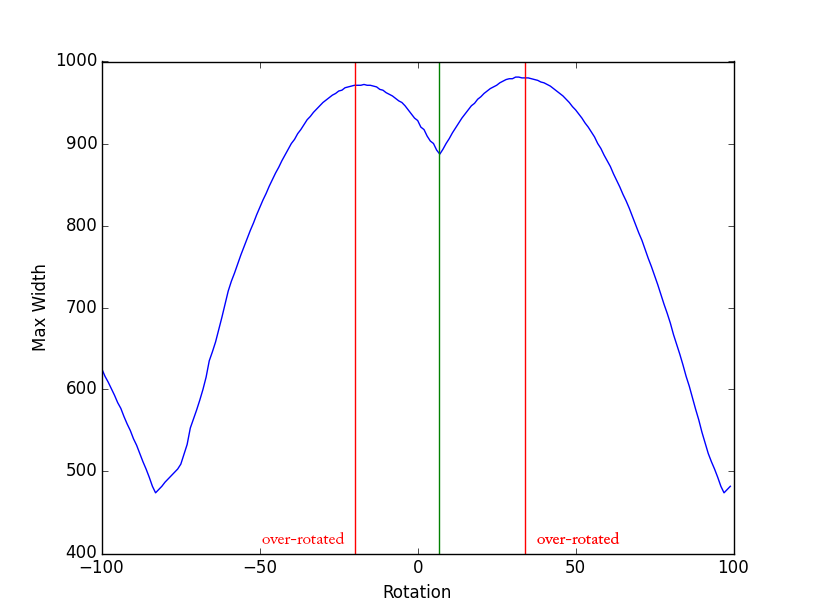
\includegraphics[width=3.2in]{rotationPlot.png}
  \caption{Encapsulating bounding box widths as a function of rotation for a short and wide document rotated -7$^\circ$, green line corresponds to desired left to right and top to bottom orientation}
  \label{fig:rotations}
\end{figure}

Technical documents contain information formatted in a rectangular shape with the left, right, top, and bottom margins defining the general structure of this rectangle. If the document were to be rotated, the rectangular form of the document context would also be rotated by the same amount. This leads to the intuition that a left to right and top to bottom oriented bounding box that contains all of a documents context would a minimum when the document is also in a left to right and top to bottom orientation. If the document were not in said orientation, then the width of the encapsulating bounding box would be some diagonal of the rectangular structure of the document's contents. Naturally, if the rectangular structure of the contents of a document had a greater width than height, the left to right and top to bottom orientation would not yield a global minimum for the width of the encapsulating bounding box. Figure \ref{fig:rotations} demonstrates such a case. The figure shows that when the image is rotated by large values, the wide and short bounding box of the proper orientation is rotated into a thin and tall bounding box which then yields smaller values for the width. This problem is addressed by taking into consideration the fact that the document images are generated with an understanding of the proper orientation of the document. Thus the probability that a document image will contain a large rotational error is very low and it is reasonable to assume that the rotation of the document will not greatly vary from the optimal orientation. In such cases, the rotation error will be such that using gradient descent to find the local minimum bounding box width will yield the optimal left to right and top to bottom rotation. Figure \ref{fig:rotations} demonstrates this fact, all points between the two red lines will result in the proper local minimum when gradient descent is used.

In order to rotate an image without accidentally cropping the image, the output image size is first specified to be a square with side length equal to the maximum value between the image width and height. The an empty image of this output size is then created and the original document image is translated such that its center is aligned with the center of the new image. This image is then rotated around its center by the desired amount. Defining the homogenized coordinates image matrix as $I$, the rotation amount to be $\theta$, the original image width to be $w$, the original image height to be $h$, and the homogenized image coordinates rotated image matrix to be $I'$ the specified transformation is given by:

\begin{align*}
\alpha &= \cos \theta \\
\beta &= \sin \theta
\end{align*}
\begin{align*}
T &= 
\left[
\begin{matrix}
1 & 0 & {\max(w,h) - w\over{2}} \\
0 & 1 & {\max(w,h) - h\over{2}} \\
0 & 0 & 1
\end{matrix}
\right]
I \\
I' &= 
\left[
\begin{matrix}
\alpha & \beta &  (1 - \alpha - \beta){\max(w,h)\over{2}}\\
-\beta & \alpha & (1 - \alpha + \beta){\max(w,h)\over{2}} \\
0 & 0 & 1
\end{matrix}
\right]
T
\end{align*}

In accordance with our findings, the algorithm for finding the correct document orientation utilizes  gradient descent to find the rotation of the document that results in a local minimum of the encapsulating bounding box width.  A bounding box containing the contents of the document is first constructed using methods similar to those discussed in section 3.2.2. Defining $\theta$ to be a rotation angle and the encapsulating bounding box width after a rotation of $\theta$ to be $W_{\theta}$, an approximation of the derivative of the bounding box width with respect to the rotation angle is given by:
\begin{align*}
{W_{\theta - \delta} - W_{\theta + \delta}\over{2\delta}}
\end{align*}
where $\delta$ represents a slight difference in rotation angle. Since the algorithm operates under the assumption that the document is not rotated by an extreme value, this derivative is first calculated for a rotation of 0 to determine whether increasing or decreasing the rotation will yield a smaller bounding box width. The algorithm then continues increasing or decreasing the rotation until the bounding box width stops decreasing. At this point the local minimum bounding box width has been located and with it the rotation that yields the left to right and top to bottom orientation of the document image. Applying this rotation to the document image thus yields a properly oriented document image which can be used for accurate data extraction.

\subsubsection{Text and Equation Sectioning}
In order to accurately extract the content of a document from the document image, the sections of the document that contain meaningful information must first be identified. Once these sections are located, a hierarchical approach is used in order to obtain fine granularity bounding boxes from which data can be accurately extracted.

The first step in this document sectioning is to identify which areas of the document image contain data and which areas of the document are meaningless background. In order to achieve this result a grayscale representation of the document image is obtained. A general horizontal and vertical Sobel operator is then applied to this grayscale image in order to obtain an image representation that focuses on the edges of the characters in the document. The intuition for this step follows from the idea that characters are very edge heavy figures and consequently areas of a document containing characters can be identified by looking for areas of the document with a large density of edges. Following the application of the Sobel operator, the image is binarized using a threshold. A standard close morphology transformation, a dilation followed by an erosion, is then used in order to connect previously identified edges present in the image. At this point our image representation will consist of large white blocks which correspond to the areas of the image containing meaningful information with the rest of the image being black. Identifying the contours in the image then allows us to obtain bounding boxes containing the desired sections of the document. During the contour finding, bounding boxes with small areas are discarded as these correspond either to meaningless artifacts in the document image or characters in the image which do not contain important information, e.g. page numbers. Steps in this process are shown in Figures \ref{fig:paper1}, \ref{fig:paper2}, and \ref{fig:paper3}.

\begin{figure}[h]
  \centering
    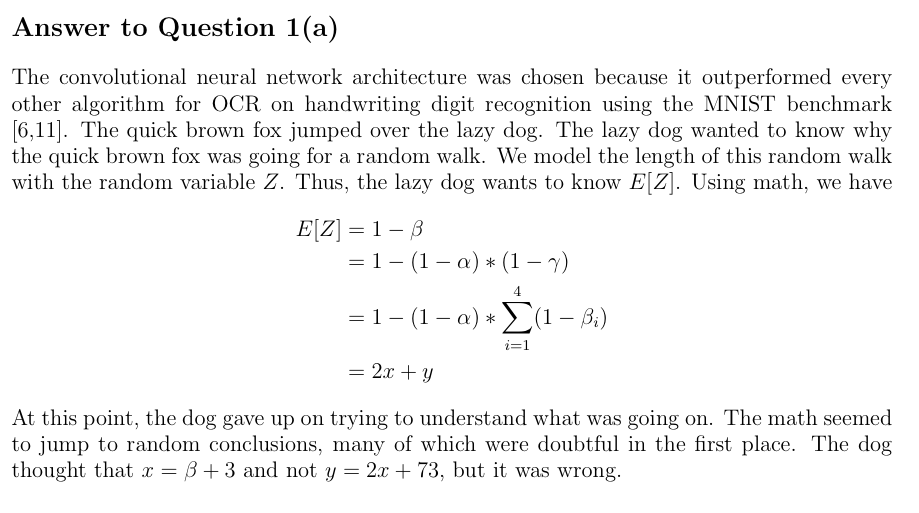
\includegraphics[width=3.2in]{paper1.png}
  \caption{Original document image.}
  \label{fig:paper1}
\end{figure}

\begin{figure}[h]
  \centering
    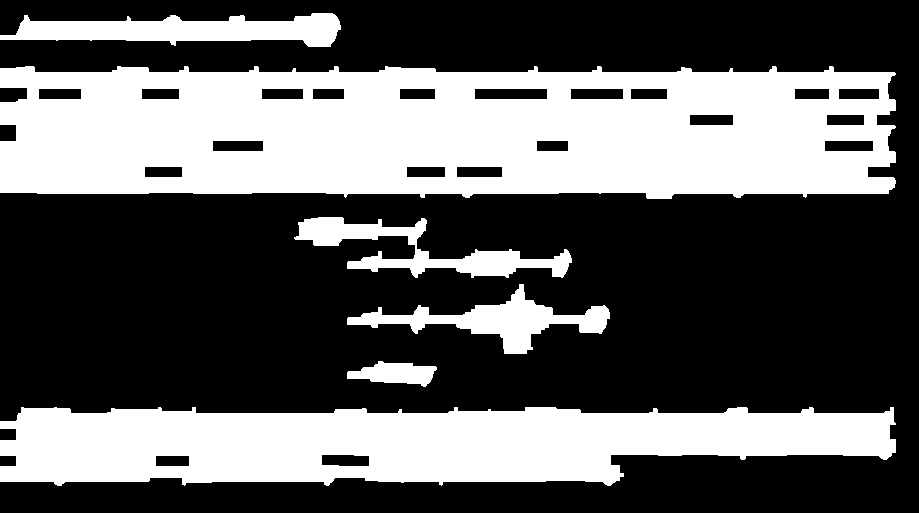
\includegraphics[width=3.2in]{paper1-morph.png}
  \caption{Document image after processing and close morphology transformation.}
  \label{fig:paper2}
\end{figure}

\begin{figure}[h]
  \centering
    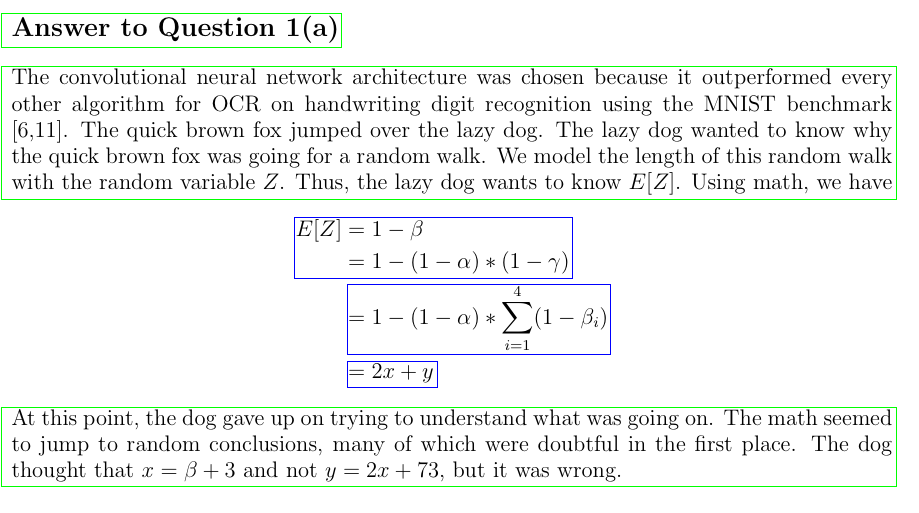
\includegraphics[width=3.2in]{paper1-bounds.png}
  \caption{Content bounding boxes in document image, text is represented by green boxes and equation blocks are represented by blue boxes}
  \label{fig:paper3}
\end{figure}

Following the identification of document sections containing information, the algorithm next classifies the obtained bounding boxes as corresponding to either display mode equation blocks or plain text paragraphs. The classification process focuses on the location of the left edge of the bounding box and classifies bounding boxes that are aligned near the left margin of the document as text while other bounding boxes are classified as equation blocks.

Given a section of an image corresponding to a block of equations, the goal of the algorithm is then to separate this equation block into its component equations. This is accomplished using a method similar to the higher level document sectioning but with a finer granularity. First the equation block image is scaled to a standard width of 700 pixels and a grayscale representation is generated. A Gaussian Blur is then applied to this grayscale representation in order to slightly increase the size of the characters in the equations while maintaining the spacing between them. This results in an increased cohesiveness between the entities of a single equation without significantly decreasing the spacing between separate equations. A Laplace operator is then applied to obtain tracings of the equations and the image is binarized using a threshold. Following the intuition that the entities in an equation are contained in approximately the same line, a strong horizontal close morphology transform is applied to the thresholded image in order to link the characters of each equation. At this point, finding contours yields bounding boxes that completely contain the vast majority of equations, however, disconnected objects such as numerators will be contained in their own individual bounding boxes. This can be remedied by extending the bounding boxes found so far to contain a large portion of the horizontal line that encapsulates the bounding box and filling in the extended bounding boxes before finding contours again. Since entities in each equation are relatively in line with each other but separate equations have vertical separation between them, extending the bounding boxes and joining them will connect the disconnected equation components without connecting separate equations. Steps in this process are shown in Figures \ref{fig:eqblock1}, \ref{fig:eqblock2}, and \ref{fig:eqblock3}.

\begin{figure}[h]
  \centering
    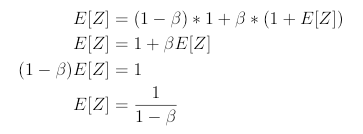
\includegraphics[width=3.2in]{eqblock1.png}
  \caption{Original equation block.}
  \label{fig:eqblock1}
\end{figure}

\begin{figure}[h]
  \centering
    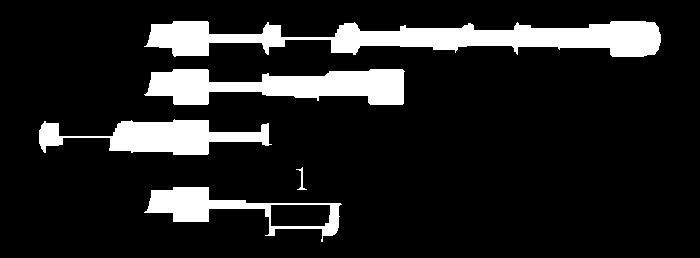
\includegraphics[width=3.2in]{eqblock1-morph.png}
  \caption{Equation block after processing and close morphology transformation.}
  \label{fig:eqblock2}
\end{figure}

\begin{figure}[h]
  \centering
    
\includegraphics[width=3.2in]{eqblock1-morph2.png}
  \caption{Equation block after bounding box extension and fill}
  \label{fig:eqblock3}
\end{figure}

The primary objective when segmenting text blocks is to segment the previously located paragraphs into bounding boxes containing each individual word. This is accomplished by first segmenting the paragraph into lines, and then segmenting the lines into words. Paragraphs are segmented into lines in a similar manner to how equation blocks are separated into equations. The paragraph image is scaled to a standard width of 700 pixels after which the image is converted to grayscale and a Gaussian Blur is applied. Applying a Laplace operator, threshold, and then strong horizontal close morphology transform yields blocks that correspond to the lines in the paragraph. The bounding boxes of these contours then define the locations of these lines. The key difference when segmenting lines into words is that the spacing between words in a line is horizontal whereas the spacing between lines in a paragraph is vertical. Thus a line image is first standardized to a height of 20 pixels before being converted to grayscale. A Laplace operator is then applied followed by a threshold and then a strong vertical and slight horizontal close morphology transform. The slight horizontal component of the close morphology closes the spaces between characters in the word while the strong vertical component guarantees that the words are represented by solid blocks in the line. Locating the spaces between the resulting blocks allows the algorithm to construct bounding boxes for each word in the line.

TODO(lshort) ADD SOME EQUATIONS. Sobel, Laplacian, Gaussian?

\subsubsection{Text Analyzing}

The lowest level of our system is a character recognizer which can classify various symbols. Our current implementation supports alphabetical, numeric, and Greek letters; common punctuation, parentheses, and brackets; and common math symbols such as $+$, $=$,  $\le$, $\sum$, $\int$, $\partial$, and $\sqrt{\cdot}$. The goal of the character recognizer is to, given a bounding box of some symbol, classify the symbol and return a key containing the appropriate \latex string. This is used to determine the characters that make up an individual word, which we will discuss later in this section, and the symbols that are in mathematical expressions, which will be discussed in Section 3.2.4.

Given a bounding box around a character, our classifier first constructs a feature vector corresponding to the image. We implemented two methods of extracting feature vectors from characters. The first approach is fairly straightforward; we start by scaling the box to be a $20 \times 20$ square and then simply use the pixel values as features. To do so, we convert the image to a ``binary'' format by applying a threshold. The dark pixels which make up the character are considered to be ``on'' pixels represented by a $1$. White pixels are represented as $0$. Thus, we can describe each character by its pixel values using a feature vector in $\mathbb{R}^{400}$ comprised of $1$s and $0$s. Since these vectors are very sensitive to the location of the character itself within its bounding box (i.e. slight translations of the character may produce very different feature vectors), we standardize this by cropping the given bounding box even further to be as small as possible and tightly wrapped around the image. This is done before scaling to $20 \times 20$ pixels. Note that this additional cropping necessarily means that this type of feature vector is invariant to the size of the letter, which has implications we discuss in Section 4.

The second approach to extracting a feature vector from a character image is adapted from what is presented in \cite{2}. For simplicity, our feature vector used $10$ of the $16$ attributes discussed by Frey and Slate. Some of the attributes were not applicable to our system, while others were too complex for the scope of our project. For example, since we standardize the height of each line to be $20$ pixels before segmenting into words and characters, the ``height'' attribute of the image is of little use to us. We noticed that the value range of each attribute varied greatly, so we scaled each attribute to lie approximately within the range $[0,15]$, similar to what was done in \cite{2}. That is, during training, we first recorded the maximum and minimum value for each attribute and then used this range to scale each value.

We trained our classifier on hundreds of images of individual characters while varying the resolution, size, and orientation of each symbol. We experimented with many different types of models used in machine learning, such as $k$-nearest neighbors ($k$-NN), SVMs, logistic regression, and decision trees. Ultimately, we decided to focus on two models -- $k$-NN and logistic regression -- since, in addition to classifying the character, these models also provided a ``score'' that indicated the confidence of the prediction. A confident classification would yield small distances in $k$-NN and high probabilities in logistic regression. The importance of having a ``score'' will be discussed in a few paragraphs.

Thus, after segmenting paragraphs into individual words using the methods in Section 3.2.2, the final step is to segment each of these words into characters so that our character recognizer can classify them. This final segmentation is one of the more difficult parts to implement, since it is sensitive to even the slightest variation in character resolution and/or spacing. We tried two main approaches to solve the character segmentation problem, each with its own benefits and drawbacks.

The first approach involves applying transformations to the image of the word, similar to what was done at the paragraph- and line-level in Section 3.2.2. To handle images with lower resolution, we first apply a Gaussian Blur and close morphology transform in order to ensure that the pixels within a character are indeed connected. The challenge arises due to the fact that characters in the same word are packed very tightly with little whitespace in between, so our Gaussian Blur and close morphology transform are very small to avoid gluing two characters together. For example, at our standard height of $20$ pixels, we found that the $(3,3)$ kernel seemed to do best for our blur. Finally, we apply a weak threshold to attempt to remove any small artifacts from the word image, and then we proceed to draw contours and bounding boxes. Figure~\ref{fig:wordBounds1} shows an example of successful character segmentation using transformations.

\begin{figure}[h]
  \centering
    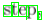
\includegraphics[width=1.5in]{word3-bounds.png}
  \caption{Successful segmentation of ``\texttt{step,}''.}
  \label{fig:wordBounds1}
\end{figure}

Our second approach is an adaptation of the slice method explored in \cite{1}. In \cite{1}, Jacobs et al. break up words into 2-pixel slices, and various combinations of slices are concatenated together to potentially form characters. In our approach, we use this as motivation and implement a sliding window algorithm that scans the word horizontally. The intuition builds off the fact that our models provide a ``score'' of confidence for each classification, and we assume our classifier is robust enough to yield high scores for images of actual characters. First, we assume that the width of any symbol must fall within the range of $2$ to $15$ pixels. Then, starting at the beginning of the word, we call our classifier on all bounding boxes of integer width $w$ between $2$ and $15$. Thus, each size bounding box yields a classification value and score, and so we pick the width $w'$ (and corresponding value) that yields the highest score. Under the assumption that text characters in paragraphs do not overlap horizontally, we then move our window forward by $w'$ to find the next character. Below is an approximate outline of our sliding window procedure, with Figure~\ref{fig:wordWindow1} providing a visual example of what occurs.

\begin{enumerate}
\item Initialize $x \leftarrow 0$.
\item Get $(\text{key},\text{score})$ of all bounding boxes with horizontal length spanning $[x, x+w]$ for all widths $w \in \{2,3,4,\dots,15\}$.
\item Let $w'$ be the width producing the best score.
\item Record key corresponding to $w'$.
\item $x \leftarrow x + w'$
\item Repeat steps 2-4 while $x <$ wordWidth.
\end{enumerate}

\begin{figure}[h]
  \centering
    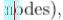
\includegraphics[width=1.5in]{word1-window.png}
  \caption{The sliding window segments the beginning \texttt{n} in ``\texttt{nodes),}''. Boxes in light blue are all possible tested bounding boxes; the line in red yielded the highest score.}
  \label{fig:wordWindow1}
\end{figure}

\subsubsection{Learning \latex Expression Layout}

Transforming images of single line mathematical expressions requires us to not only recognize individual symbols used in the expression, but also the layout of the expression. To perform this, we used a simplified version of the method used in \cite{4}, which we will now describe in detail. 

The first step in transforming a mathematical expression to \latex markup is to classify each individual symbol in the expression. This is done by calling upon our character recognizer discussed in Section 3.2.3. The character recognizer gives, or classifies, each bounding box with a key which contains the appropriate \latex string for the symbol. Once symbols are matched with the individual \latex strings, the next step is to learn the structure of the expression to assemble theses strings together in a coherent fashion.
 
To do this, we work with a few more attributes of each symbol. Each bounding box of a symbol is described by four values, $x_m$, $y_m$, $w$ and $h$, where $x_m$ and $y_m$ denote the $(x,y)$ coordinates of the top-left corner of the box and $w$ and $h$ denote the width and height of the box. Coordinates of pixels in the image have $x$ values that increase from left to right and $y$ values that increase from top down.

For each bounding box detected in the image for an expression, we define three additional values. The \textit{centroid} of a symbol is a point in the bounding box that indicates, roughly, where the center of the symbol lies. The \textit{sup-threshold} of a symbol denotes the upper bound for the $y$ value of a superscript, while the \textit{sub-threshold} denotes the lower bound for the $y$ value of a subscript. Figure~\ref{fig:values} gives a visual representation for each of these definitions. 

Each symbol is categorized as one of three types: \textit{ascendant}, \textit{descendant}, \textit{central}. These distinctions allow us to distinguish characters that are imbalanced in the $y$ direction. For example, characters like $\partial$ and $b$ are ascendant symbols, $\gamma$ and $p$ are descendant symbols, and $c$ and $\int$ are central symbols. Based on the type of the symbol, we compute the values for the centroid, sup-threshold, and sub-threshold differently, as shown in Table \ref{tab:values}. These values, together with $x_m$, $y_m$, $w$ and $h$ are used to compare locations between symbols, which we explain next.

\begin{figure}[h]
  \centering
    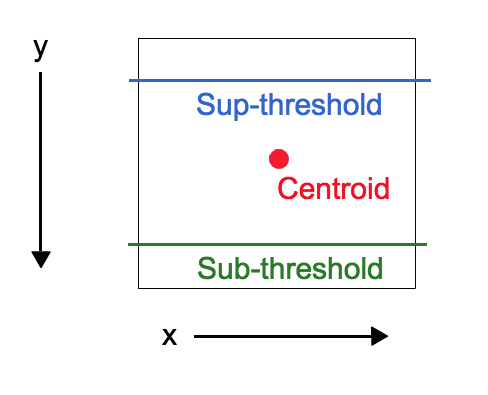
\includegraphics[width=3.2in]{values.png}
  \caption{Points and lines of interest for a bounding box}
  \label{fig:values}
\end{figure}

\begin{table}[h]
  \caption{centroid and threshold values for different symbol types}
  \centering
  \begin{tabular}{l l l l}
  \hline
  & centroid $y$ & sup-threshold & sub-threshold\\
  \hline
  ascendant & $y_m + 0.66h$ & $y_m + 0.2h$ & $y_m+0.8h$\\
  descendant & $y_m+ 0.33h$ & $y_m +0.1h$ & $y_m+0.4h$\\
  central & $y_m+0.5h$ & $y_m+0.25h$ & $y_m+0.75h$\\
  \hline
  \end{tabular}
  \label{tab:values}
\end{table}

One of the main ideas presented in \cite{4} is the concept of dominance. Each symbol is capable of dominating some subset of five different regions: \textit{above}, \textit{below}, \textit{superscript}, \textit{subscript}, and \textit{subexpression}. Tapia and Rojas define a few additional regions in \cite{4}, but for the sake of simplicity, the five regions we have defined cover all of the symbols we currently support. The locations of each of these regions, relative to the bounding box, is show in Figure~\ref{fig:locations}. A symbol $A$ is said to dominate a symbol $B$ if $B$ lies in one of the regions dominated by $A$, and $B$ does not exceed $A$ in both width and height. 
\begin{figure}[h]
  \centering
    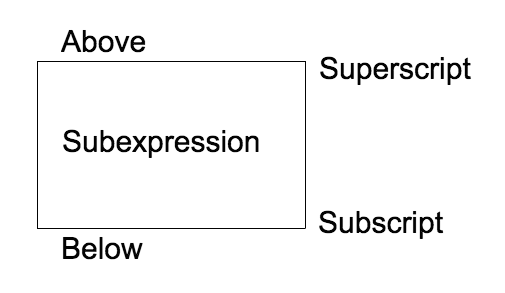
\includegraphics[width=3.2in]{locations.png}
  \caption{Dominated regions of a symbol}
  \label{fig:locations}
\end{figure}

Now, given the image of the expression and the bounding box for each symbol, we wish to learn the \latex layout of the symbols. For example, consider the following expression
\[ \sum_{n = -\infty}^\infty \left|\left\langle f, \frac{e^{inx}}{\sqrt{2\pi}} \right\rangle \right|^2 = \|f\|^2 \] 


\begin{figure*}[h]
\centering
\pgfdeclarelayer{bg}    % declare background layer
\pgfsetlayers{bg,main}  % set the order of the layers (main is the standard layer)
\begin{tikzpicture}
[dot/.style={rectangle,draw=black,fill=white,inner sep=5pt,minimum size=5pt}]
\node[dot] at (0,12) (n0) {root};
\node[dot] at (-8,10) (n1) {\verb$\sum$};
\node[dot] at (-6.5,10) (n2) {\verb$|$};
\node[dot] at (-4.5,10) (n3) {\verb$\langle$};
\node[dot] at (-2.5,10) (n4) {\verb$f$};
\node[dot] at (-1.5,10) (n5) {\verb$,$};
\node[dot] at (0,10) (n6) {\verb$\frac$};
\node[dot] at (2.25,10) (n7) {\verb$\rangle$};
\node[dot] at (4,10) (n8) {\verb$|$};
\node[dot] at (5,10) (n9) {\verb$=$};
\node[dot] at (6,10) (n10) {\verb$\|$};
\node[dot] at (7,10) (n11) {\verb$f$};
\node[dot] at (8,10) (n12) {\verb$\|$};
\node[dot] at (-8,8) (n13) {above};
\node[dot] at (-6,8) (n14) {below};
\node[dot] at (-1,8) (n15) {above};
\node[dot] at (1,8) (n16) {below};
\node[dot] at (4,8) (n17) {supscr};
\node[dot] at (8,8) (n18) {supscr};
\node[dot] at (-8,6) (n19) {\verb$\infty$};
\node[dot] at (-6.5,6) (n20) {\verb$n$};
\node[dot] at (-5.8,6) (n21) {\verb$=$};
\node[dot] at (-5,6) (n22) {\verb$-$};
\node[dot] at (-3.5,6) (n23) {\verb$\infty$};
\node[dot] at (-1,6) (n24) {\verb$e$};
\node[dot] at (1,6) (n25) {\verb$\sqrt$};
\node[dot] at (4,6) (n26) {\verb$2$};
\node[dot] at (8,6) (n27) {\verb$2$};
\node[dot] at (-1,4) (n28) {supscr};
\node[dot] at (1,4) (n29) {subexp};
\node[dot] at (-2,2) (n30) {\verb$i$};
\node[dot] at (-1,2) (n31) {\verb$n$};
\node[dot] at (0,2) (n32) {\verb$x$};
\node[dot] at (1,2) (n33) {\verb$2$};
\node[dot] at (2.25,2) (n34) {\verb$\pi$};

\begin{pgfonlayer}{bg}    % select the background layer
\draw[-] (n0) -- (n1);
\draw[-] (n0) -- (n2);
\draw[-] (n0) -- (n3);
\draw[-] (n0) -- (n4);
\draw[-] (n0) -- (n5);
\draw[-] (n0) -- (n6);
\draw[-] (n0) -- (n7);
\draw[-] (n0) -- (n8);
\draw[-] (n0) -- (n9);
\draw[-] (n0) -- (n10);
\draw[-] (n0) -- (n11);
\draw[-] (n0) -- (n12);
\draw[-] (n1) -- (n13);
\draw[-] (n1) -- (n14);
\draw[-] (n6) -- (n15);
\draw[-] (n6) -- (n16);
\draw[-] (n8) -- (n17);
\draw[-] (n12) -- (n18);
\draw[-] (n13) -- (n19);
\draw[-] (n14) -- (n20);
\draw[-] (n14) -- (n21);
\draw[-] (n14) -- (n22);
\draw[-] (n14) -- (n23);
\draw[-] (n15) -- (n24);
\draw[-] (n16) -- (n25);
\draw[-] (n17) -- (n26);
\draw[-] (n18) -- (n27);
\draw[-] (n24) -- (n28);
\draw[-] (n25) -- (n29);
\draw[-] (n28) -- (n30);
\draw[-] (n28) -- (n31);
\draw[-] (n28) -- (n32);
\draw[-] (n29) -- (n33);
\draw[-] (n29) -- (n34);
\end{pgfonlayer}
\end{tikzpicture}
  \caption{\latex markup tree}
  \label{fig:latexTree}
\end{figure*}

The actual \latex markup corresponding to this expression can be broken down into a tree structure, shown in Figure~\ref{fig:latexTree}. To learn this tree structure, we first find the \textit{dominant baseline} of symbols, which consists of all of the children of the root node. These are the primary symbols in our \latex expression that are not dominated by any other symbols, and in general will have centroids that lie roughly on the same line. To find this baseline, we find the most dominant expression, defined as the expression with the largest bounding box perimeter that is not dominated by any other expressions. In our example expression, the most dominant expression is given by the summation symbol. We then compute the centroid of the most dominant expression and find all other dominant expressions with centroids that have similar $y$ coordinates. Figure~\ref{fig:baseline} shows the bounding boxes and the baseline symbols for the example expression.

\begin{figure}[h]
  \centering
    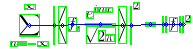
\includegraphics[width=2in]{equation2-baseline.png}
  \caption{Baseline symbols}
  \label{fig:baseline}
\end{figure}

Once the dominant baseline is established, the centroids of the nodes in the baseline are connected from left to right to form a line structure. All remaining symbols are attached to the baseline nodes using Prim's algorithm for minimum spanning trees. For each branch of the spanning tree connected to the baseline, this process of finding the most dominated symbol, followed by finding the dominant baseline, and lastly constructing the minimum spanning tree is recursively repeated. Ultimately, this yields a tree like the one in Figure~\ref{fig:spanningTree}. The recursive layering of this algorithm naturally produces well-defined parent-child relationships between the nodes of the tree. For each parent symbol, child nodes in same dominated regions are grouped together as sibling nodes, which allows us to construct the \latex tree in Figure~\ref{fig:latexTree}. From the tree, we can construct the appropriate \latex markup string, since children either serve as arguments, superscripts, or subscripts of their parents. 

\begin{figure}[h]
  \centering
    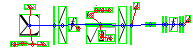
\includegraphics[width=2in]{equation2-mst.png}
  \caption{Final spanning tree of symbols}
  \label{fig:spanningTree}
\end{figure}

\subsubsection{Latex Construction}

TODO(crwong, dzeng - Math if not in 3.2.4)

\section{Experimentation Results}

$\alpha\beta\gamma\delta\epsilon\varepsilon\zeta\eta\theta\iota\kappa\lambda\mu\nu\xi\pi\rho\sigma\tau\upsilon\phi\chi\psi\omega$
agg

\section{Conclusion}

aggabla

\begin{thebibliography}{1}
\bibitem{1} C. Jacobs, P. Simard, P. Viola, J. Rinker. Text Recognition of Low-resolution Document Images. Microsoft, 2005.
\bibitem{2} P. Frey, D. Slate. Letter Recognition Using Holland-Style
Adaptive Classifiers. Machine Learning, 1991. \\
\bibitem{3} G. Gupta, S. Niranjan, A. Shrivastava. Document Layout Analysis \& Classification and Its Application in OCR. EDOCW, 2006. \\
\bibitem{4} E. Tapia, R. Rojas. Recognition of On-line Handwritten Mathematical Expressions Using a Minimum Spanning Tree Construction and Symbol Dominance. LNCS, 2004.
\end{thebibliography}

%\balancecolumns

\end{document}
